\documentclass[11pt]{article}
\usepackage[top=1in,bottom=1in,left=1in,right=1in]{geometry}
\usepackage{amsfonts}
\usepackage{graphicx}
\usepackage{float}
\usepackage[nottoc,notlot,notlof]{tocbibind}
\usepackage{tikz}
\usepackage{array}
\usepackage[utf8]{inputenc}
\usepackage[english]{babel}
\usepackage{hyperref}
\usetikzlibrary{shapes.geometric,arrows}
\tikzstyle{process} = [rectangle,minimum width=3cm, minimum height=1cm, text centered,draw=black, fill=orange!30]
\tikzstyle{arrow}=[thick,->,>=stealth]

\usepackage{fancyhdr}
\pagestyle{fancy}
\fancyhead{}
\fancyfoot{}
\fancyhead[C]{\slshape\MakeUppercase{Design of Radial vane Impeller}}
%\fancyhead[R]{\slshape Aditya Amatya}
\fancyfoot[C]{\thepage}

\parindent 0ex
%\setlength{\parindent}{4em}
%\setlength{parskip}{1em}
\renewcommand{\baselinestretch}{1.5}

\begin{document}
\begin{titlepage}
\begin{center}

\includegraphics[scale=.5]{TU.png}\\
\centering
\vspace*{.5cm}
  \Large\textbf{TRIBHUVAN UNIVERSITY} \\
  \Large\textbf{INSTITUE OF ENGINEERING} \\
    \Large\textbf{CENTRAL CAMPUS PULCHOWK} \\
  \vfill
  \line(1,0){400}\\
 \Large{\textbf{A \\REPORT\\ ON\\ DESIGN AND ANALYSIS OF RADIAL VANE IMPELLER}}\\[0.1cm]

 \line(1,0){400}\\
 \vfill
 SUBMITTED BY :\\
  ADITYA AMATYA\\
 072BME603\\
 \vfill
 SUBMITTED TO :\\
 DEPARTMENT OF MECHANICAL ENGINEERING\\
 LALITPUR NEPAL\\
 \vfill
 \today
\end{center}
\large
\end{titlepage}

\tableofcontents
\thispagestyle{empty}
\clearpage
\listoffigures
\thispagestyle{empty}
\clearpage

\setcounter{page}{1}

 \section{Introduction}
 \subsection{Centrifugal Fan}
Centrifugal fans are a dynamic axisymmetric,work-absorbing turbo machinery which are used to transport fluids by the conversion of rotational kinetic energy to the hydrodynamic energy of the fluid flow. The rotational energy typically comes from an engine or electric motor.\\
It increases the pressure of an incoming air stream by impellers, a series of blades mounted on a circular hub, which in turn accelerates air radially and alters the direction of the outward flowing air, usually by 90$^\circ$ . As centrifugal fans are constant volume devices that create steadier flow of air than axial fans, they are most widely used in various industrial processes such as in transporting air/gas and material handling.
In centrifugal flow, airflow changes direction twice - once when entering and second when leaving.
  \subsubsection{Impeller}
 Impellers are rotating component of turbo machines like compressors, fans  usually made of iron, steel, bronze, brass, aluminum or plastic, which transfers energy from the motor that drives the pump to the fluid being pumped by accelerating the fluid outwards from the center of rotation.\\
Impellers consist of various vanes arranged around a central shaft.As the impeller rotates, the fluid is drawn into the blade passage at the impeller eye, the center of the impeller. The inlet pipe is axial and therefore fluid enters the impeller with very little whirl or tangential component of velocity and flows outwards in the direction of the blades. The fluid receives energy from the impeller while flowing through it and is discharged with increased pressure and velocity.\\
 \subsection{Plug Fan}
A plug fan is a single inlet, free blowing fan, where the unit casing functions as fan housing.\\
Plug fan is also a centrifugal fan but it is mounted in different way.The plug fan is mounted without volute casing.There is a plate on which motor bearing arrangement is supported carrying the drive shaft. Impeller is mounted in the drive shaft.\\
Compared to traditional centrifugal fans, plug fans offer lower energy consumption and lower costs, resulting in much shorter payback periods and increased operating efficiency.\\ 
The plug fan has an efficiency of up to 75\%.
 
\subsubsection{Types of Centrifugal Fans}

Based on blade configuration centrifugal fans are broadly divided into four different types.They are as follows:-
\begin{enumerate}
\item Radial blade Fan
\item Forward Curved Blade Fan
\item Backward Curved Blade Fan
\item Airfoil Blade Fan 

\end{enumerate}

\textbf{Radial blade Fan}\\
These are high-pressure fans with medium airflow. Radial-bladed fans are best for industrial applications where there is dust, or in environments where there is gas or moisture in the air.\\
\textbf{Forward Curved Blade Fan}\\
These are medium pressure, high airflow fans that can be used in both clean air, ventilating and exhaust applications.\\
\textbf{Backward Curved Blade Fan}\\
These are high-pressure, high flow, high efficiency fans. Power reduces as flow increases over the most efficient area of the system.\\
\textbf{Airfoil Blade Fan}\\
These are the highest efficiency fans, best in clean air applications.\\

\begin{figure}[h!]
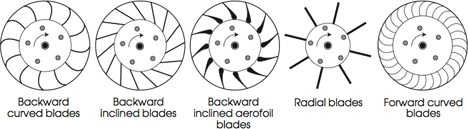
\includegraphics[scale=1]{fans.png}
\caption{Types of Fans}
\end{figure}
\clearpage
The max. efficiency of each type of fans along with its application are as follows :- \\
\begin{figure}[h!]
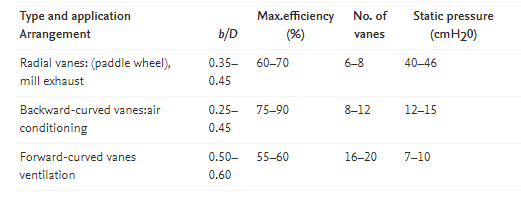
\includegraphics[scale=1]{efficiency.png}\\
\centering
\caption{Maximum Efficiency of fan}
\end{figure}

\subsection{Fundamental Equation and Velocity diagram of Radial Vane Blade}
Radial blade centrifugal fans also called as paddle wheel fans, consists of an impeller with multiple equally spaced flat blades that are extending perpendicular to the direction of wheel rotation. The wheel is a paddle type wheel which may or may not contain side rims and the blades are comparatively heavier, deeper and narrower than forward and backward inclined blades.They produce medium to high pressure and moves relatively a higher mass or volume of fluid.\\
If a mass $m$ rotates about an axis at radius $r$ , and at a tangential velocity,$V$ , then it has an angular momentum of $mrv$. Furthermore, if the mass is a fluid that is continuously being replaced then it becomes a mass flow $\frac{dm}{dt}$ , and a torque $T$,must be maintained that is equal to corresponding continuous rate of change of momentum$$T=\frac{dm}{dt}(rv)$$
In the case of centrifugal impeller , the peripheral component of fluid velocity is $C_u$.Hence, the torque becomes
$$T=\frac{dm}{dt}(rC_u)$$
The increase angular momentum due to the mass of elemental fluids across the inlet and outlet locations in time $dt$ is
$$T=\frac{dm}{dt}(r_2C_{u2}-r_1C_{u1})$$
Also,
$$\frac{dm}{dt} = Q\rho$$
where $Q$ = volume of flow ($m^3/s$)\\
 $\rho$ = fluid density($kg/m^3$)\\
 Hence,\\
 $$ T= Q\rho[r_2C_{u2}-r_1C_{u1}]$$
        Now,the power consumed by the impeller, $P_{ow}$ is equal to the rate of doing mechanical work,
        $$P_{ow} =T\omega$$
        where, $\omega$ is speed of rotation ($rad/s$)\\
        giving, 
        $$P_{ow} =Q\rho\omega[r_2C_{u2}-r_1C_{u1}]$$
        $$P_{ow} =Q\rho[u_2C_{u2}-u_1C_{u1}]$$\\
        Where, $\omega r_2=u_2$ is tangential velocity at outlet\\
         $\omega r_1=u_1$ is tangential velocity at inet\\
       The Power imparted by a fan impeller to the air is $P_{ft}Q$\\
       where $P_{ft}$= rise in total pressure across the fan.
       In the absence of frictional or shock losses,$P_{ft}Q$ must equal the power consumed by the impeller, $P_{ow}$.Hence,
       $$P_{ft}=Q\rho[u_2C_{u2}-u_1C_{u1}]$$
       This relationship gives the theoretical fan total pressure and is known as \texttt{Euler's Equation.}\\
       Euler's equation can be written as 
       $$P_{ft}=\rho \left\lbrace\frac{{u_2}^2-{u_1}^2}{2}-\frac{{W_2}^2-{W_1}^2}{2}-\frac{{C_2}^2-{C_1}^2}{2}\right\rbrace$$
       
       Finally, the equation for pressure rise is given by
       $$P_{ft}=A-BQ$$
       
       where constants \\$$ A = \rho {u_2}^2$$
       and \\
       $$B=\frac{\rho u_2}{a_2tan\beta_2}$$
       
       For radial blade $\beta_2 = 90^\circ$ and $\tan\beta_2 =\infty$\\
       giving $B=0$\\
       Then ,
       $$P_{ft}=A =\rho {u_2}^2$$
       which implies theoretically, Pressure remains constant at all the flows.\\
\begin{figure}[h!]
\centering
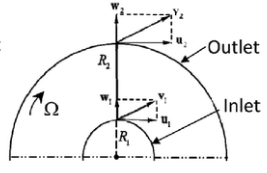
\includegraphics[scale=1]{velocity.png}\\
\caption{Velocity diagram of radial Blade}
\end{figure}
       
 \subsection{Historical Background}
 The earliest mention of centrifugal fans was in 1556 by Georg Pawer (Latin: Georgius Agricola) in his book De Re Metallica, where he shows how such fans were used to ventilate mines. Thereafter, centrifugal fans gradually fell into disuse. It wasn’t until the early decades of the nineteenth century that interest in centrifugal fans revived. In 1815 the Marquis de Chabannes advocated the use of a centrifugal fan and took out a British patent in the same year. In 1827, Edwin A. Stevens of Bordentown, New Jersey, installed a fan for blowing air into the boilers of the steamship North America. Similarly, in 1832, the Swedish-American engineer John Ericsson used a centrifugal fan as blower on the steamship Corsair. A centrifugal fan was invented by Russian military engineer Alexander Sablukov in 1832, and was used both in the Russian light industry (such as sugar making) and abroad.

One of the most important developments for the mining industry was the Guibal fan, which was patented in Belgiumin 1862 by the French engineer Théophile Guibal. The Guibal fan had a spiral case surrounding the fan blades, as well as a flexible shutter to control the escape velocity, which made it far superior to previous open-fan designs and led to the possibility of mining at great depths. Such fans were used extensively for mine ventilation throughout Britain.\\
Some of the leading companies manufacturing these kinds of fans are Atlas Copco ,Rotating Machinery Services, Inc. ,Elliott Company,Sundyne Corporation,FS-Elliott Co. LLC .
 \subsection{Applications}
 \textbf{Radial blade types} are well suited for material handling and in some moderate pressure industrial applications.\\
 \textbf{Backward curved fans} are typically used in low pressure, high volume applications such as heating, ventilation and air conditioning systems.\\
 \textbf{ Forward curved fans} has delicate construction of the impeller, shaft, bearings, and housing and thus limits its suitability in industrial applications. These fans are ideal for low speed and low pressure applications such as in domestic furnaces, central station units, packaged air conditioning etc.\\
 \textbf{Airfoil blade fans} can handle large volumes of air,these fans are extensively used in forced and induced draft fans that are suitable for broad operating ranges in industrial applications,H VAC systems, air pollution control, drying  and filtration, and other industrial processes.

 \section{Methodology}
 The radial vane impeller is designed based on some preliminary assumptions as well as some provided design parameters like thickness of channel,thickness of blade,radius of impeller eye,radius of outlet,etc.Certain mathematical calculations is done using theoretical formula for radial impeller discussed above.Speed of impeller is assumed to be $1200 rpm$ and density of air is assumed to be $1.225 kg/m^3$.\\
 These calculations are used to plot the performance chart in EXCEL.
 After 1D calculations , 2D drawing is done using Solidworks which were used to design the 3D model of Impeller.3D design software  CATIA is used to design the 3D model of radial vane Impeller. These 3D models were imported in ANSYS workbench. The proper meshing is done there and final simulation is done using CFX environment.Different contours were visualized along with comparison of results from simulations and 1D calculations.\\
 The flowchart for the methodology is as follows:-\\
 \begin{center}
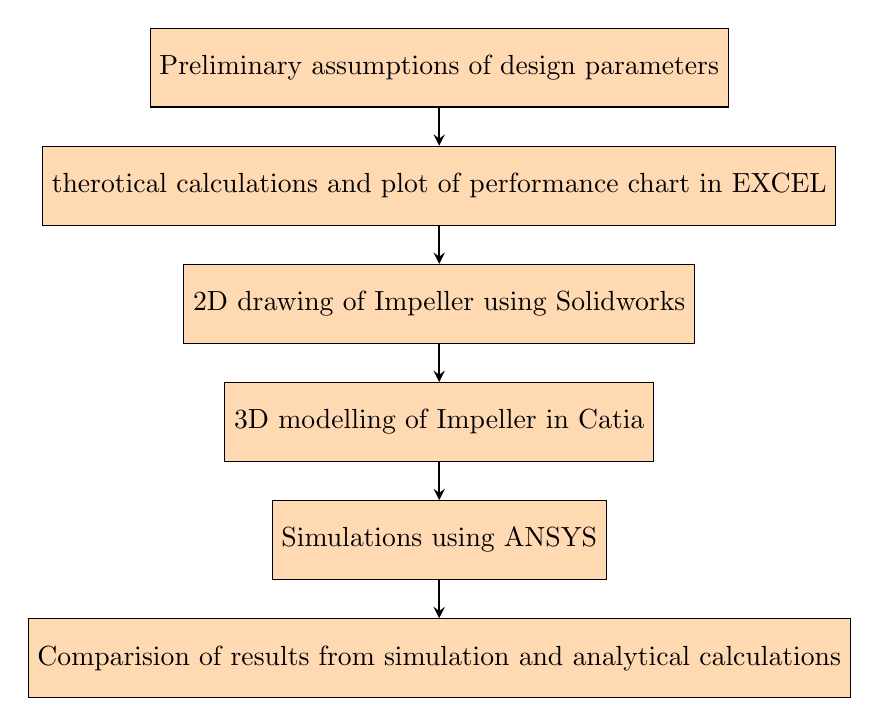
\begin{tikzpicture}[node distance=1.5cm]
\node(first)[process]{Preliminary assumptions of design parameters};
\node(second)[process,below of=first]{therotical calculations and plot of performance chart in EXCEL};
\node(third)[process,below of=second]{2D drawing of Impeller using Solidworks};
\node(fourth)[process,below of=third]{3D modelling of Impeller in Catia};
\node(fifth)[process,below of=fourth]{ Simulations using ANSYS };
\node(sixth)[process,below of=fifth]{Comparision of results from simulation and analytical calculations};

\draw[arrow](first)--(second);
\draw[arrow](second)--(third);
\draw[arrow](third)--(fourth);
\draw[arrow](fourth)--(fifth);
\draw[arrow](fifth)--(sixth);
\end{tikzpicture}
\end{center}

The design parameters used for analytical calculations as well as modelling of Impeller are as follows:-\\
\begin{table}[]
\centering
\begin{tabular}{|c|c|c|c|}
\hline
Student Roll No.                                  & 603                        & Blade thickness(mm)                              & 3                      \\ \hline
$R_{in}$(mm)                                           & 303                        & $\beta 1 $                                  & $90^\circ$ \\ \hline
$R_{out}$(mm)                                          & 506                        &$\beta 2 $                                   &$90^\circ$ \\ \hline
Hub and Shroud Thickness(mm)                      & 10                         & Impeller Thickness(mm)                           & 100     \\ \hline
No. of Blades                                     & 8                          & Speed of Impeller(rpm)                           & 1200    \\ \hline
\multicolumn{1}{|l|}{Atmospheric density (kg/m3)} & \multicolumn{1}{l|}{1.225} & \multicolumn{1}{l|}{Inlet axial flow velocity(m/s)} & \multicolumn{1}{l|}{2} \\ \hline
\end{tabular}
\caption{Preliminary Design Parameters}
\end{table}
\subsection{1D Design}
 The Euler's equation gives the theoretical fan total pressure which is as follows 
 $$P_{ft}=Q\rho[u_2C_{u2}-u_1C_{u1}]$$ 
 Applying the calculations from velocity triangle of radial impeller ,finally, Euler's equation becomes as follows \\
  $$P_{ft}=\rho \left\lbrace\frac{{u_2}^2-{u_1}^2}{2}-\frac{{W_2}^2-{W_1}^2}{2}-\frac{{C_2}^2-{C_1}^2}{2}\right\rbrace$$\\
  
 This equations explains that the rise in pressure or say change in pressure in centrifugal fan is due to centrifugal effect , relative velocity effect and change in kinetic energy of fluid.\\
 In other words, change in pressure is sum of gain in static pressure and gain in velocity pressure.\\
 Eulers's equation may be employed to develop pressure-volume relationships for centrifugal impeller.\\
  
  The performance chart plotted in EXCEL using the analytical calculations using are as follows :-\\
  
 \begin{figure}[h!]
\centering
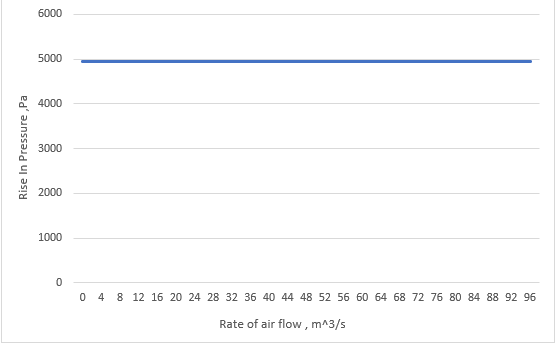
\includegraphics[scale=1]{pvsq.png}\\
\caption{Performance chart of Pressure rise vs flow-rate}
\end{figure}

\begin{figure}[h!]
\centering
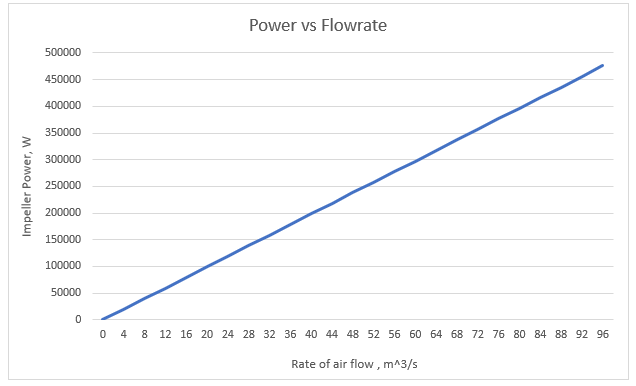
\includegraphics[scale=1]{povsq.png}\\
\caption{Performance chart of Power vs flow-rate}
\end{figure}
Speed of impeller is assumed to be $1200 rpm$ and density of air is assumed to be $1.225 kg/m^3$.The $\beta$ is by default $90^\circ$ for radial vane Impeller.
The table for this performance chart is as follows :- \\
\begin{table}[]
\centering
\begin{tabular}{|c|c|c|c|}
\hline
S.N. & Rate of airflow (Q ), m\textasciicircum{}3/s & Rise in Pressure(Pft), Pa & Impeller Power (Pow) ,W \\ \hline
1    & 0                                            & 4956.85696                & 0                       \\ \hline
2    & 4                                            & 4956.85696                & 19827.42784             \\ \hline
3    & 8                                            & 4956.85696                & 39654.85568             \\ \hline
4    & 12                                           & 4956.85696                & 59482.28352             \\ \hline
5    & 16                                           & 4956.85696                & 79309.71136             \\ \hline
6    & 20                                           & 4956.85696                & 99137.1392              \\ \hline
7    & 24                                           & 4956.85696                & 118964.567              \\ \hline
8    & 28                                           & 4956.85696                & 138791.9949             \\ \hline
9    & 32                                           & 4956.85696                & 158619.4227             \\ \hline
10   & 36                                           & 4956.85696                & 178446.8506             \\ \hline
\end{tabular}
\caption{Analytical Calculations result}
\end{table}
\subsection{3D Design}
 The fully constrained orthographic view of the radial vane impeller is as follows :-\\
\begin{figure}[H]
\centering
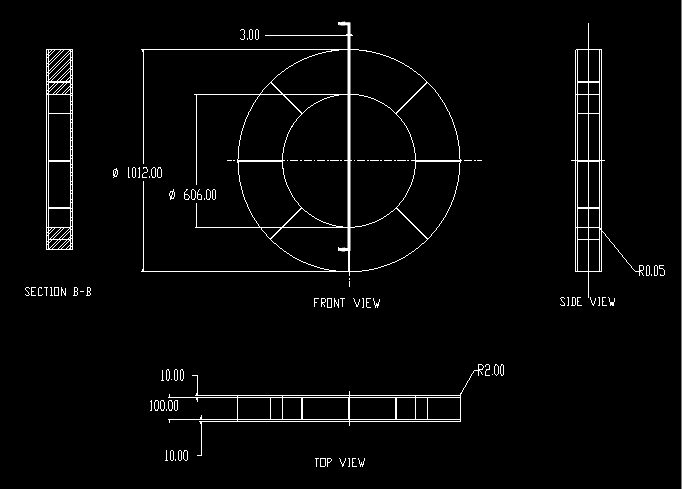
\includegraphics[scale=.6]{orthographic.png}\\
\caption{Orthographic Views of Radial vane Impeller}
\end{figure}
\clearpage
The isometric view of 3D cad model is as follows:\\
 \begin{center}
 \begin{figure}[hbt!]
 \centering
 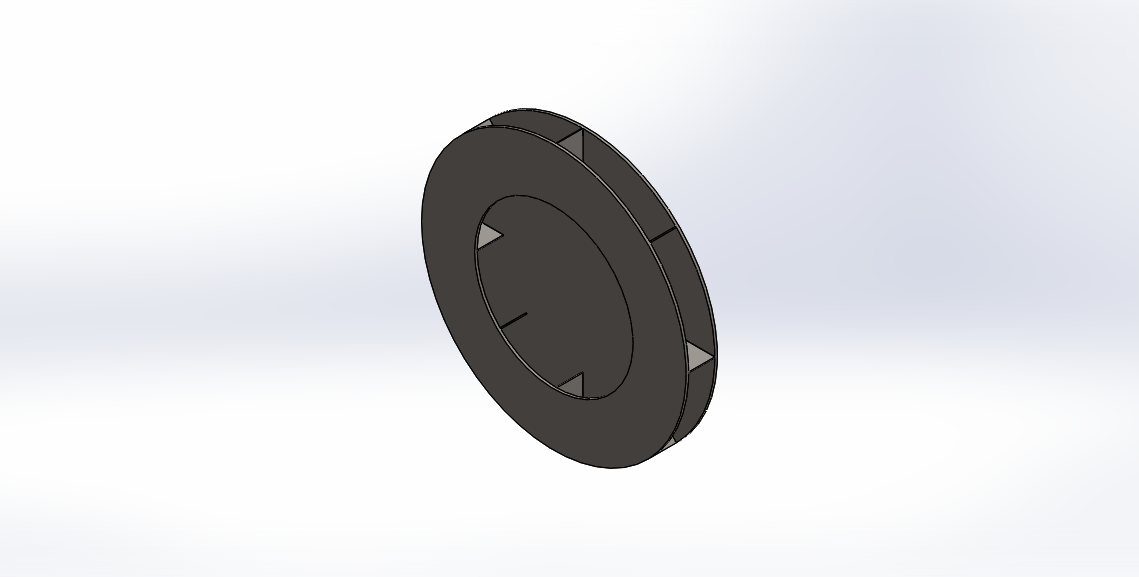
\includegraphics[scale=.5]{isometric.png}\\
 \caption{Isometric view of Radial vane Impeller}
 \end{figure}
 \end{center}
\begin{center}
 \begin{figure}[hbt!]
 \centering
 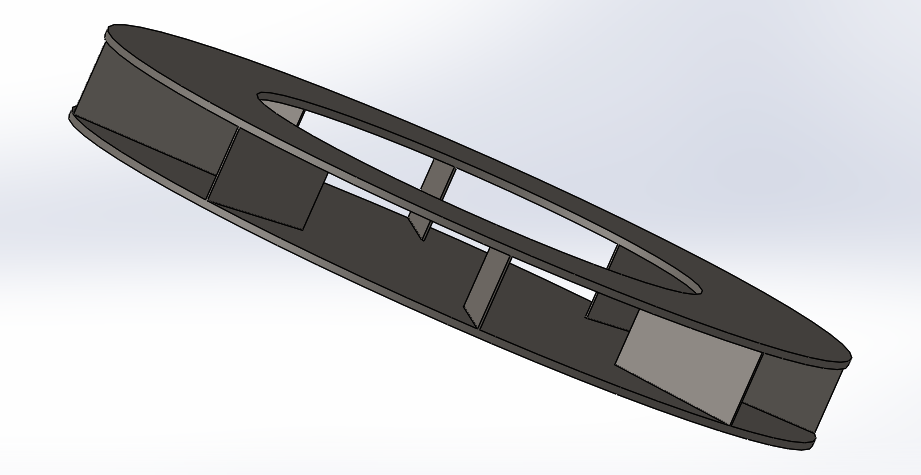
\includegraphics[scale=.6]{isometric2.png}\\
 \caption{Isometric view of Radial vane Impeller}
 \end{figure}
 \end{center}

\subsection{CFD Simulation}
In a CFD analysis, the examination of fluid flow in accordance with its physical properties such as velocity, pressure, temperature, density and viscosity is conducted. To virtually generate a solution for a physical phenomenon associated with fluid flow, without compromise on accuracy, those properties have to be considered simultaneously.\\
A mathematical model of the physical case and a numerical method are used in a software tool to analyze the fluid flow.\\
In this project ANSYS CFX solver is used for CFD simulation.
\subsubsection{Geometry}
 The overall geometry  used in this simulation are of three kinds.They are inlet, outlet and rotor.It is done in-order to define the domain of fluid during simulations.Inlet is the part through which fluid enters into rotor.Similarly,fluid is expelled out through outlet.Rotor is the part where fluid's pressure and velocity changes due to energy of blade.Since, the behavior of fluid is different at these three different part.So, separate geometries are made for inlet,rotor and outlet.\\
 For Rotor ,two separate part i.e. blade tool and rotor domain is made, which then gets subtracted using boolean in design modeler. It is done in order to make proper domain for fluid.The Blade gets subtracted here ,which provides the actual space or domain for fluid.\\
 Similarly, a sector is only used in simulation. It's done in-order to save calculation cost.Since, Centrifugal impeller is axis-symmetric,there would be no change in results using sector.It is beneficial to use sector for axis-symmetric geometry as it saves a lot of computational time.\\
 The orthographic view with detailed dimension of inlet , outlet, rotor and blade is as follows :-\\
 \begin{center}
 \begin{figure}[hbt!]
 \centering
 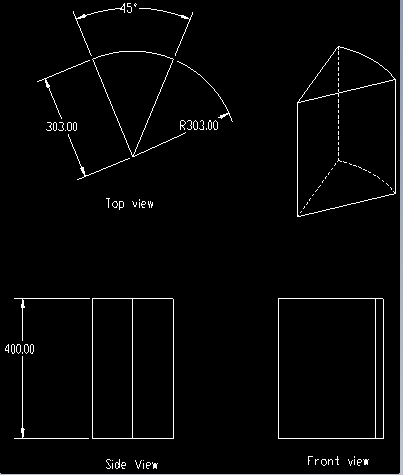
\includegraphics[scale=.6]{inlet.png}\\
 \caption{Isometric view of Inlet}
 \end{figure}
 \end{center}
 \begin{center}
 \begin{figure}[hbt!]
 \centering
 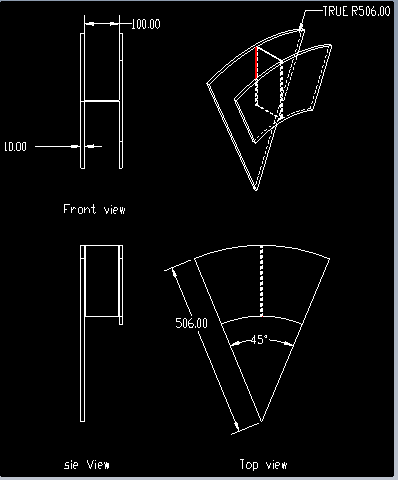
\includegraphics[scale=.6]{blade.png}\\
 \caption{Isometric view of Blade}
 \end{figure}
 \end{center}
 \begin{center}
 \begin{figure}[hbt!]
 \centering
 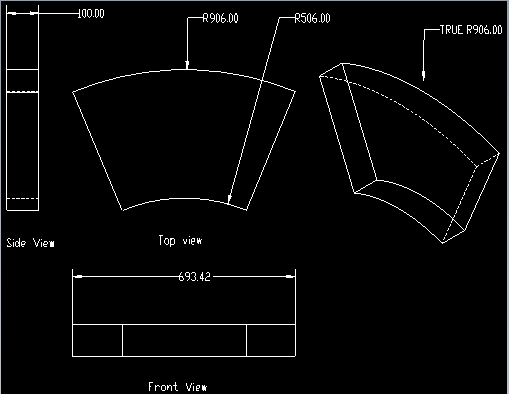
\includegraphics[scale=.6]{outlet.png}\\
 \caption{Isometric view of outlet}
 \end{figure}
 \end{center}
 
 \begin{center}
 \begin{figure}[hbt!]
 \centering
 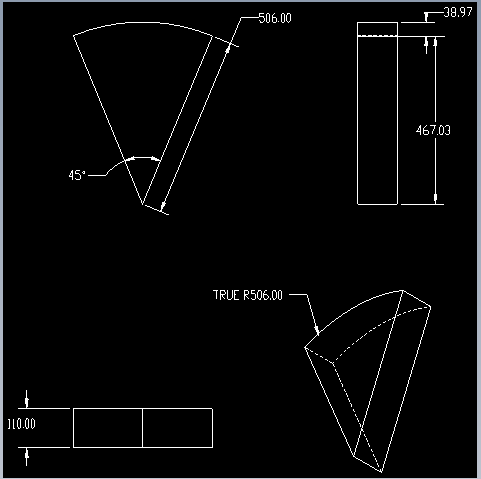
\includegraphics[scale=.6]{rotor.png}\\
 \caption{Isometric view of rotor}
 \end{figure}
 \end{center}
 \clearpage
\subsubsection{Meshing}
 
  Meshing is nothing but discretization of continuous body into finite number of elements.\\
 Since,it is CFD simulation, the physics preference is CFD and solver preference is CFX for meshing.The element are ordered linearly. 
Along with default refinement by ANSYS, face refinement is also done during the meshing of rotor.Rotor Inlet and Blade face are refined.The total number of nodes is 175971 and total number of elements in rotor is 901915.\\
The figure of mesh in rotor is as follows :-

   \begin{center}
 \begin{figure}[H]
 \centering
 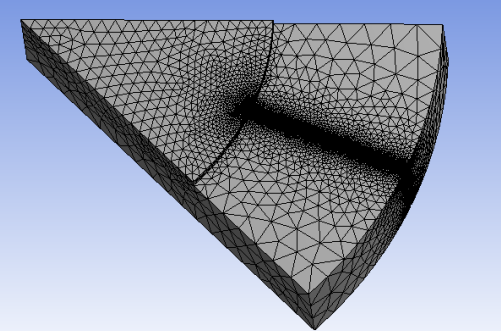
\includegraphics[scale=1]{rotormesh.png}\\
 \caption{Mesh of rotor}
 \end{figure}
 \end{center}
 
In inlet, face refinement is done at interference.Body sizing is used to control the minimum size of elements. The total number of nodes is 29646 and total number of elements in rotor is 158200.The element size is kept 0.01$m$.
   \begin{center}
 \begin{figure}[H]
 \centering
 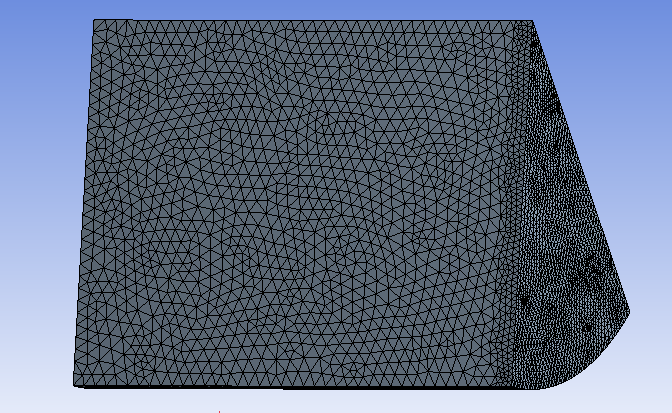
\includegraphics[scale=1]{inletmesh.png}\\
 \caption{Mesh of Inlet}
 \end{figure}
 \end{center}
  In outlet also, face refinement is done at interference.Body sizing is used to control the minimum size of elements.The total number of nodes is 2812 and total number of elements in rotor is 9249.The element size is kept 0.02$m$.
 \begin{center}
 \begin{figure}[H]
 \centering
 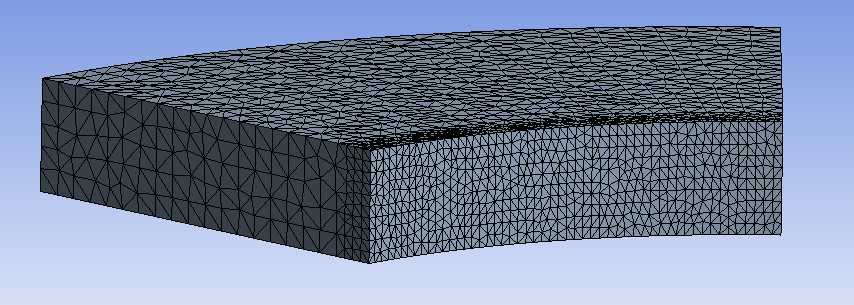
\includegraphics[scale=.6]{outletmesh.png}\\
 \caption{Mesh of Outlet}
 \end{figure}
 \end{center}

 \subsubsection{Physics Setup}
 The Physics setup is done using Turbo Mode in CFX solver.Centrifugal Compressor is chosen as machine type and analysis is done assuming steady state of flow.\\
 Inlet and Outlet is selected as stationary component and rotor is selected as rotating component and the rotational speed is $1200 rpm$.The fluid chosen is ideal air gas and reference pressure is $1 atm$.$K-epsilon$ $(k-\epsilon)$ turbulence model is chosen to simulate mean flow characteristics for turbulent flow conditions.\\
The domain interface is chosen in two face.First one is done at $Inlet-out$ and $Rotor_In$. The second interface is done at $Outlet_In$ and $Rotor_Out$.For these interface Frozen rotor type is chosen.The Frozen Rotor model treats the flow from one component to the next by changing the frame of reference while maintaining the relative position of the components. Usually, periodicity is used to reduce the number of components to a subset that has approximately the same pitch ratio as the full geometry.\\
Different boundary conditions is used to constrain the model.At $Inlet_In$ the flow is specified at normal speed of $2 ms_{-}$.Along with inlet,symmetry and wall is also used to constrain the stationary component. For rotor , symmetry and wall is used as boundary conditions.Similarly, for outlet symmetry,wall as well as outlet at $0 atm$ relative pressure is used.\\
For convergence control, 10000 is used at maximum iterations while residual target is set to $1e^{-4}$.


 \begin{center}
 \begin{figure}[H]
 \centering
 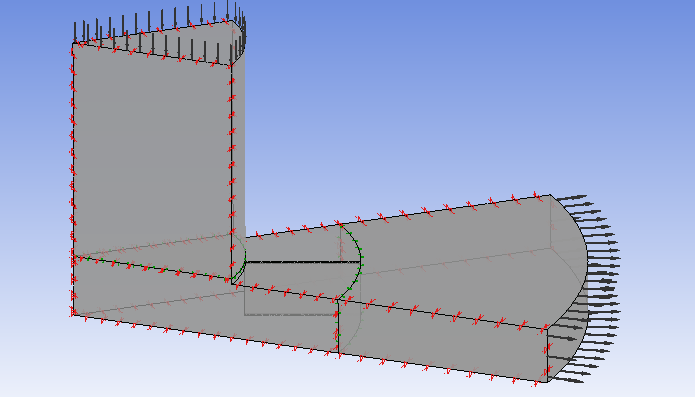
\includegraphics[scale=.6]{boundary.png}\\
 \caption{Boundary setup in CFX}
 \end{figure}
 \end{center}
 \subsubsection{Solver}
 CFX solver is used to simulate the radial vane Impeller. In CFX the solver is almost locked.It is very robust solver and rarely needs to have its default parameters changed.In the CFX, the volume of control is assembled around the nodes (Cell Vertex), where each element is divided in sub volumes. As a result, the flux through each face is based on the nodal values of element. Once subdomain contributions evaluated, nodes will accounting for each sub volume around itself and the real volume of control is assembled. In term of grid quality CFX is more permissive.\\
 \section{Results}
 Different contour plots for velocity, pressure as well as comparison of between simulation results and analytical calculations is also done in this section.
 \subsection{Contour Plot}
 \begin{center}
 \begin{figure}[H]
 \centering
 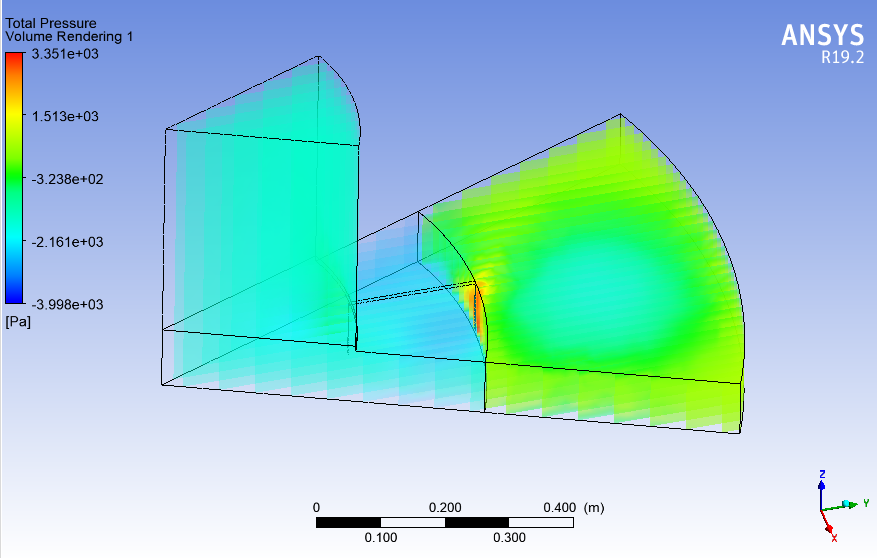
\includegraphics[scale=.6]{totalpressure.png}\\
 \caption{Rendering of total Pressure field}
 \end{figure}
 \end{center}
 \begin{center}
 \begin{figure}[H]
 \centering
 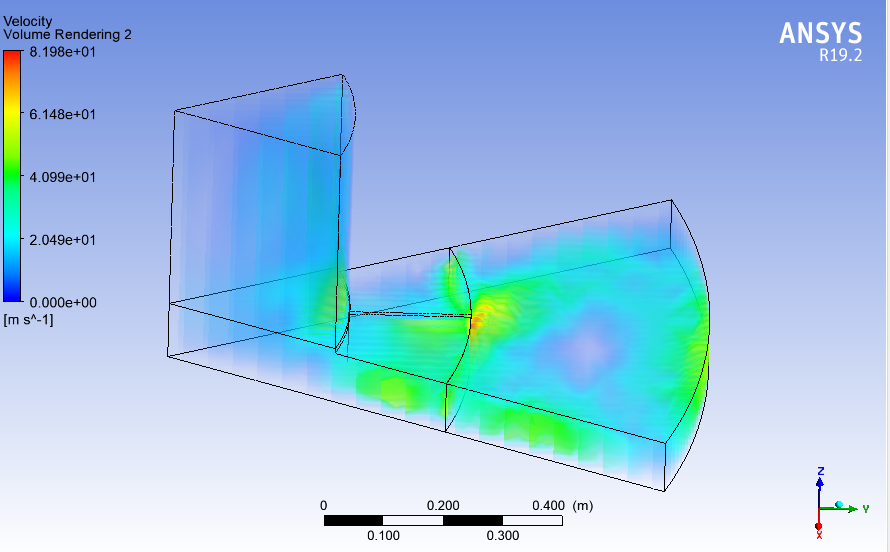
\includegraphics[scale=.6]{velocitycontour.png}\\
 \caption{Rendering of Velocity field }
 \end{figure}
 \end{center}
 \begin{center}
 \begin{figure}[H]
 \centering
 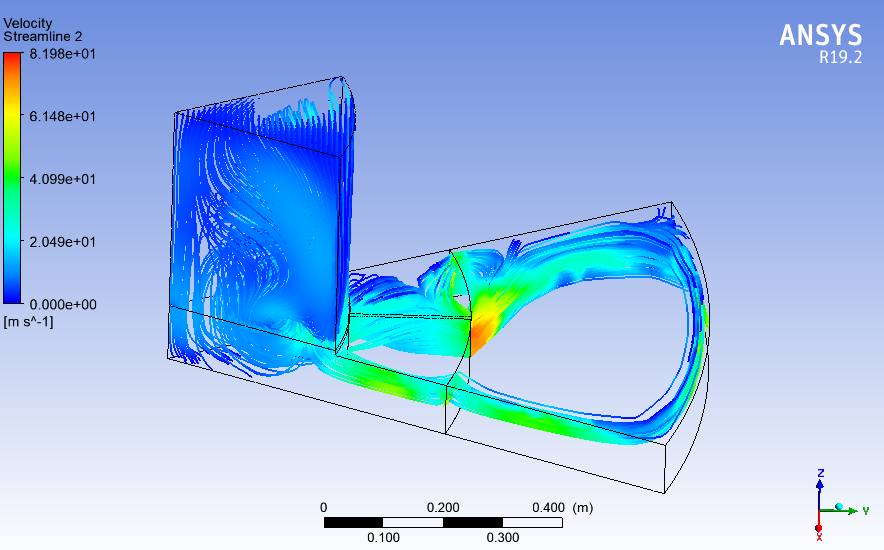
\includegraphics[scale=.6]{streamlineplot.png}\\
 \caption{Rendering Streamline}
 \end{figure}
 \end{center}
 \subsection{Result Verification}
 From 1D calculation :\\
 Pressure rise = 4956.8 Pa\\
 Torque = 22.74 N.m\\
 From Simulation results:\\
 Pressure rise = 2179.58 Pa\\
 Torque = 66.27 N.m \\
 
 \section{Conclusion and Remarks}
 The error in the calculation of pressure rise is $127.4\%$and for torque, the error is  $191.4\%$ .The meshing which ultimately affects convergence of results may be one of the factor for such kind huge error.The other factors contributing the error may be geometry of model as well as the assumptions made.\\
 CFD solver like CFX is great aid for simulating the different fans,compressor,and other turbo devices.The actual visualization along with proper calculations can be done which can be so helpful in manufacturing process.Better designs for Turbo Machines can be done by proper optimization of results using CFD.The real world machines can directly be analyzed through these kind of tools.
 
\end{document}
